% vim:sw=4:ts=4:autoindent:tw=72
% vim:sw=4:ts=4:autoindent:tw=72
\documentclass[a4paper,11pt]{report}
\usepackage[utf8]{inputenc}
\usepackage[T1]{fontenc}
\usepackage[usenames, dvipsnames]{color}
\usepackage[english]{babel}
\usepackage{amsmath,bm}
\usepackage{empheq} % rutor runt ekv
\numberwithin{equation}{chapter} 
\renewcommand{\frac}[2]{\dfrac{#1}{#2}}
\usepackage{units}
\usepackage{graphicx}
\graphicspath{{images/}}
\usepackage{bbm}
\usepackage{rotating}
\usepackage{icomma}
\usepackage{comment}
\usepackage{booktabs}
\usepackage{dsfont}
\usepackage{float}
\usepackage{subfigure}
\usepackage[a4paper, margin=3cm]{geometry}
\usepackage[font={small,it}]{caption}
\usepackage{t1enc}
\usepackage{amssymb}
\usepackage{url}
\usepackage{multicol}
\usepackage{wrapfig}
\usepackage{adjustbox}
\usepackage{wallpaper}
\usepackage[sorting=none,natbib=true,url=true]{biblatex}
\bibliography{references}
\usepackage{tabu} % använd "tabu" istället för "tabular"
\usepackage{longtable}
\usepackage{blindtext}
\usepackage{parskip}

% Typografiska rådet
% 2) 1.5 radavstånd (även om det står 1.3)
\linespread{1.3}
\usepackage[para,bottom]{footmisc}
\usepackage{hyperref}

\usepackage{appendix}

\usepackage{gensymb} 

% för sidhuvud
\usepackage{fancyhdr}
\fancypagestyle{plain}{
    \fancyhf{} % empty header and footer
    \renewcommand{\headrulewidth}{0pt} % ho header line
    \renewcommand{\footrulewidth}{0pt}% not footer line
    \fancyfoot[C]{\thepage}% like fancy style
}

% För kod
\usepackage{minted}
\newcommand{\code}[1]{\texttt{#1}}
\renewcommand\listingscaption{Lista}
\newcommand{\sgn}{\operatorname{sgn}}

% kommandon för att referera, använd dessa istället för \ref
\newcommand{\Tblref}[1]{Table~\ref{#1}}
\newcommand{\Figref}[1]{Figure~\ref{#1}}
\newcommand{\Secref}[1]{Section \ref{#1}~\emph{\nameref{#1}}}
\newcommand{\Chapref}[1]{Chapter \ref{#1}~\emph{\nameref{#1}}}
\newcommand{\Listref}[1]{List~\ref{#1}}
\newcommand{\tblref}[1]{table~\ref{#1}}
\newcommand{\figref}[1]{figure~\ref{#1}}
\newcommand{\secref}[1]{section \ref{#1}~\emph{\nameref{#1}}}
\newcommand{\chapref}[1]{chapter \ref{#1}~\emph{\nameref{#1}}}
\newcommand{\eqnref}[1]{(\ref{#1})}
\newcommand{\listref}[1]{list~\ref{#1}}

\newcommand*{\figuretitle}[1]{%
    {\centering
    #1
    \par\medskip}
}

% T0DO-kommando:
\newcommand{\todo}[1]{%
	\textbf{{\color{red} TODO: #1}}
}

% titeln på arbetet
\newcommand{\thesistitle}{Revealing relations in highly dimensional temporal data}
\newcommand{\thesissubtitle}{}


% var och när detta arbete gjordes
\newcommand{\whereandwhen}{%
	Department of Physics\\
	\textsc{Chalmers University of Technology}\\
	Göteborg, Sweden 2017\\
}

% vad är det för arbete?
\newcommand{\whatthisis}{%
	Master's thesis
}

\usepackage{pgfgantt} % För att göra Gantt-tabell
\usepackage{pdfpages} % för att inkludera pdf-fil

\begin{document}

\pagestyle{empty}
% vim:sw=4:ts=4:autoindent:tw=72
% Framsida
% OBS skilj på titelsida och framsida! se
% https://student.portal.chalmers.se/sv/chalmersstudier/kandidat-och-examensarbete/examensarbete/Sidor/utformning-rapporter-exjobb-kand.aspx

% från
% http://tex.stackexchange.com/questions/46280/how-to-create-a-background-image-on-title-page-with-latex
\ThisLRCornerWallPaper{1}{front_page.pdf}
\vspace*{3cm}
\begin{comment}
\begin{figure}[H]
\centering
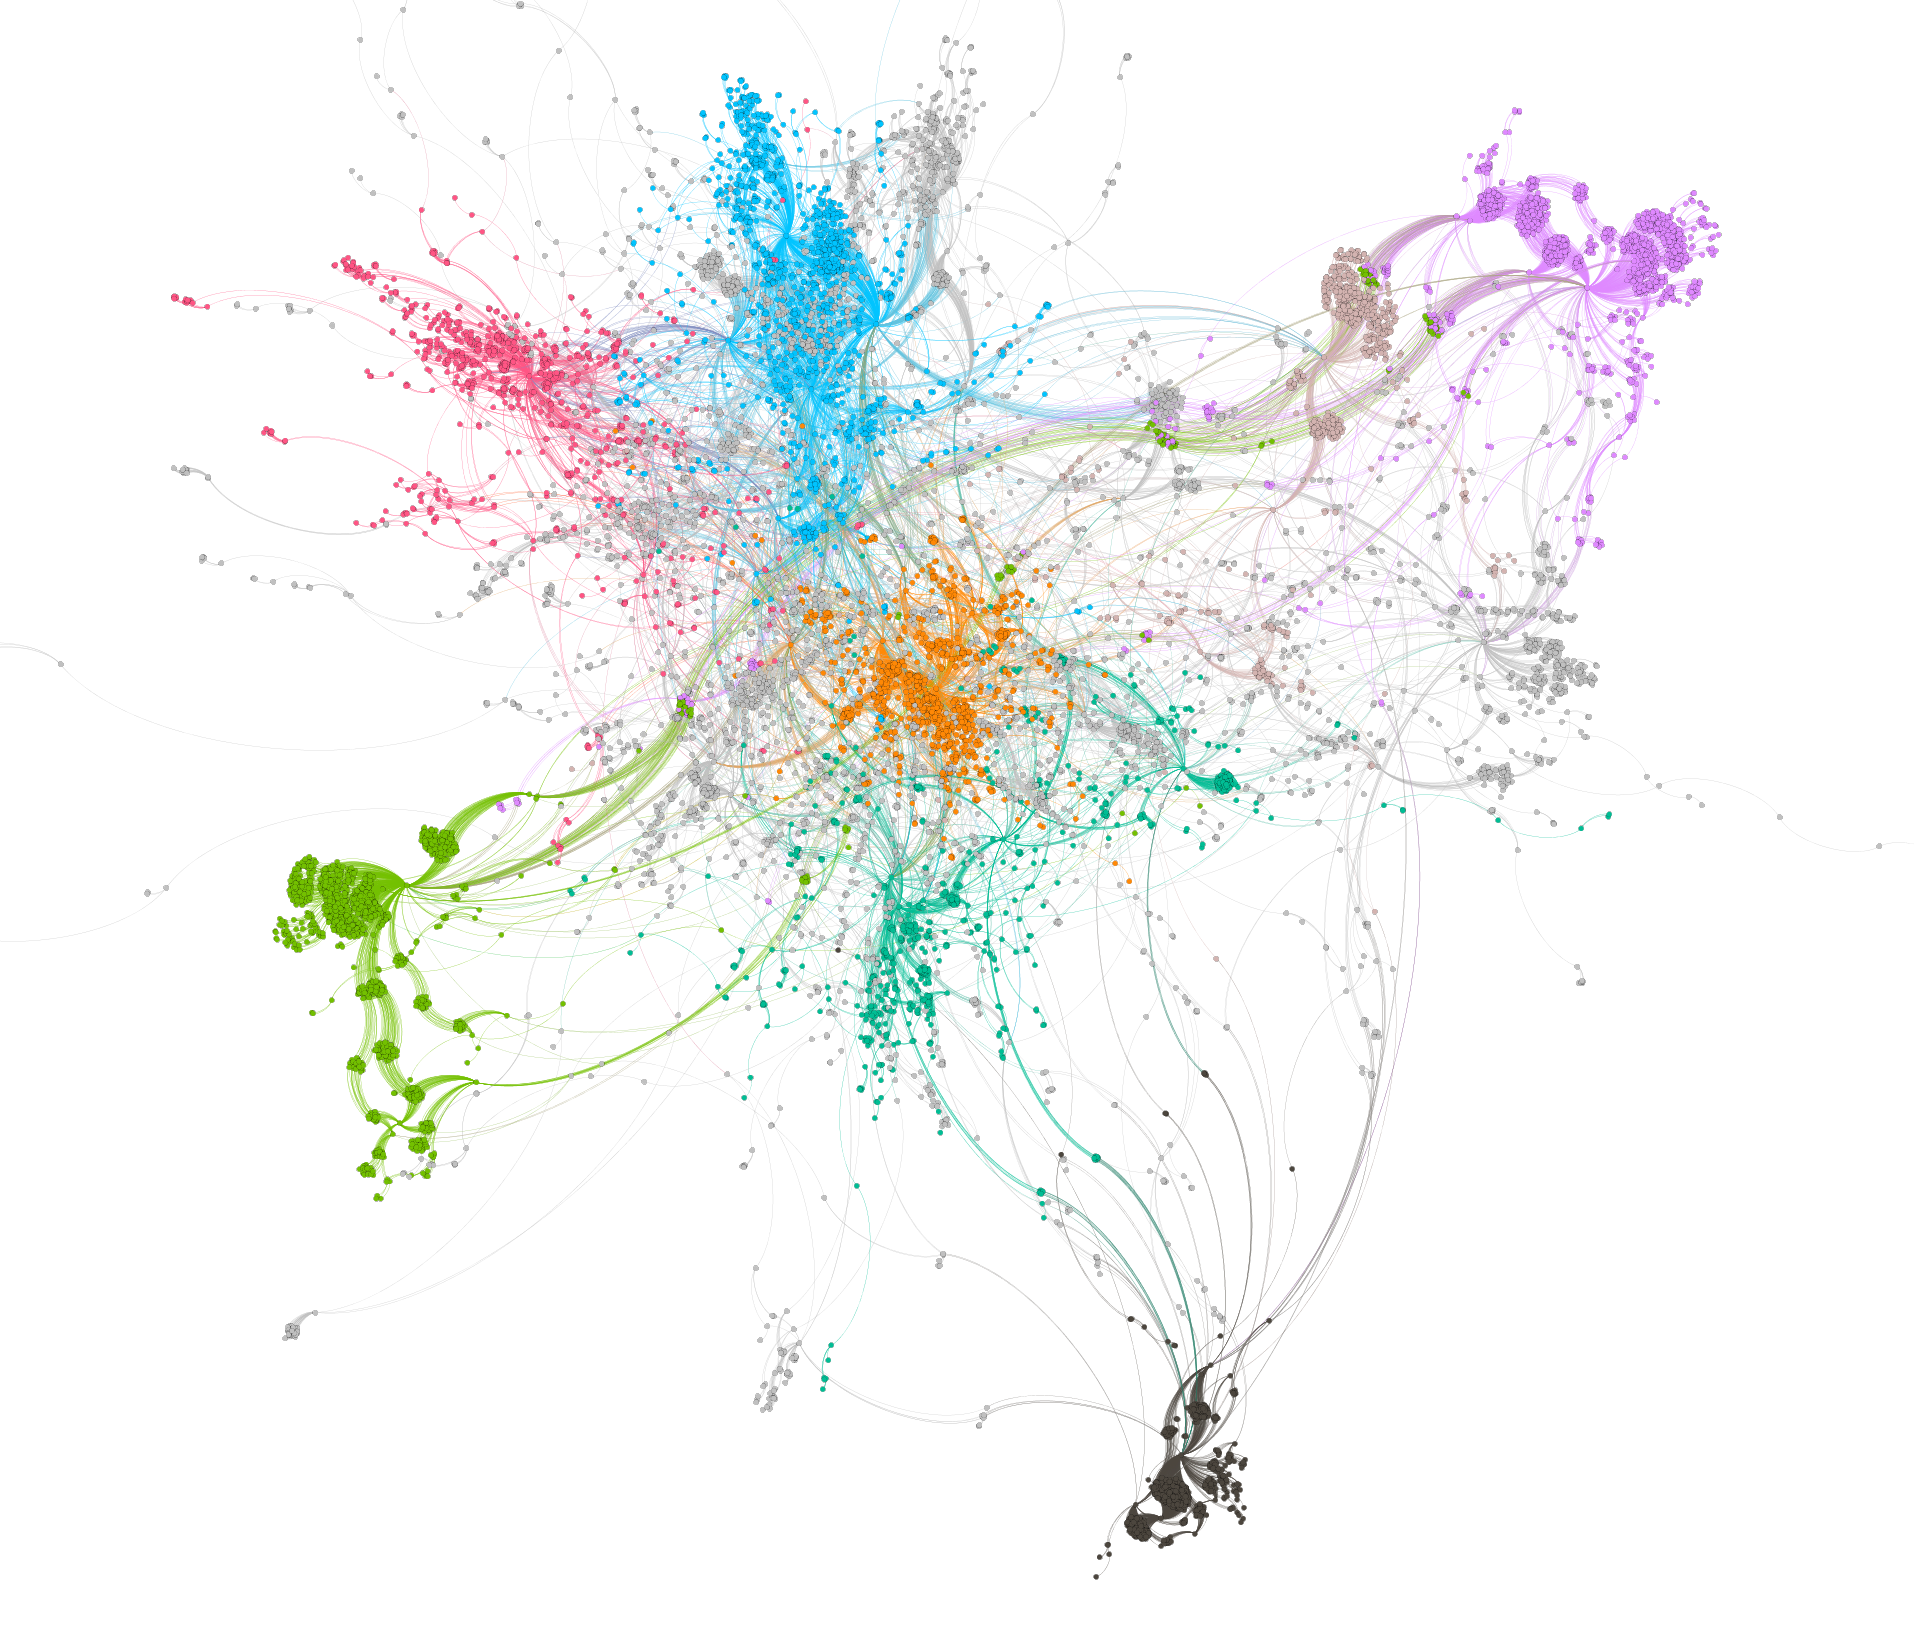
\includegraphics[width = 0.95\textwidth]{network.png}
\end{figure}
%\vspace*{\fill}
\begin{flushleft}
        \noindent{%
			% arbetstitel
			{\Huge \thesistitle} \\[.1cm]
			% undertitel

        	{\large \whatthisis}\\
        
			\bigskip
			\Large{%
				Henrik Adolfsson\\
				Josephine Cuellar Andersson\\
			}

		}
\end{flushleft}
\end{comment}

\thispagestyle{empty}
\newpage

\newpage
% vim:sw=4:ts=4:autoindent:tw=72
% Tryckortssida

\noindent
\thesistitle \\
\thesissubtitle \\
\whatthisis \\
\\
\large{%
    Henrik Adolfsson\\
	Josephine Cuellar Andersson\\
}

\vspace*{\fill}
\noindent
Image on front page:\\
Network of...

\thispagestyle{empty}
\newpage

% vim:sw=4:ts=4:autoindent:tw=72
% Titelsida
% OBS skilj på titelsida och framsida! se
% https://student.portal.chalmers.se/sv/chalmersstudier/kandidat-och-examensarbete/examensarbete/Sidor/utformning-rapporter-exjobb-kand.aspx

\begin{center}
	%\LARGE \textsc{Slutrapport}\\
	\bigskip
	\bigskip
	\Huge{Revealing relations in high \\dimensional data}\\
	\medskip
	\Large{-- BASED ON LINK PREDICTION AND NODE SIMILARITY \\IN A GRAPH} \\
\end{center}

\bigskip
\bigskip
\noindent\rule{\linewidth}{0.4pt}
\bigskip

% Taget från
% http://tex.stackexchange.com/questions/56875/how-do-i-make-one-minipage-the-same-size-as-another
\newlength\myheight
\begin{center}
	\begin{adjustbox}{%
		minipage=[t]{0.40\linewidth},
		gstore totalheight=\myheight
	}
		\begin{flushleft}
			% Namnen sorterade efter efternamn
			\large \emph{Authors:}\\
			Henrik Adolfsson\\
			\text{henado@student.chalmers.se}\\[0.3cm]
			Josephine Cuellar Andersson\\
			\text{josander@student.chalmers.se}\\[0.3cm] 
		\end{flushleft}
	\end{adjustbox}
	\hspace{0.5cm}
	\begin{adjustbox}{minipage=[t][\myheight]{0.4\linewidth}}
		\begin{flushright} \large
			\emph{Examiner:} \\
			Mats Granath\\ [0.3cm]

			\emph{Supervisors:} \\
			Staffan Truv\'e\\
			Michel Edkrantz\\
		\end{flushright}
	\end{adjustbox}
\end{center}

\vspace*{\fill}

\begin{center}
	\Large{%
		\whereandwhen
	}
\end{center}


\thispagestyle{empty}
\newpage


%%%%%%%%%%%%%%%%%%%%%%%%%%%%%%%%%%%%%%%%%%%%%%%%%%%%%%%%%%%%%%%%
% Front matter
\setcounter{page}{1}
\pagenumbering{roman}

% abstract
% vim:sw=4:ts=4:autoindent:tw=72

\noindent
\thesistitle\\
\thesissubtitle\\
\whatthisis\\
\\
\large{%
    Henrik Adolfsson\\
	Josephine Cuellar Andersson\\
}\\
\\
\large{%
	\whereandwhen
}

\vspace*{\fill}
\begin{center}
    \section*{Abstract}
\end{center}
Very interesting abstract... 
\newline
\noindent
\textbf{Key words:} graph, relations.

% toc
\newpage
\tableofcontents
\newpage

%% vim:sw=4:ts=4:autoindent:tw=72

% använd detta kommando för att lägga till ett ord
\newcommand{\wordexpl}[2]{%
	\textbf{#1}\hspace*{.2cm}#2\\
}

\chapter*{Word explanation}
\addcontentsline{toc}{chapter}{Word explanation}

% asterisk gör att vi fyller den vänstra kolumnen först
\setlength\columnsep{25pt}
\begin{multicols}{2}
\noindent
Explanation of central concepts in this report. The words might have a different meaning in other contexts.
\vspace*{.1cm}

    \noindent
    \wordexpl{Aggregation}{An aggregation of references.}
    \wordexpl{Attacker}{A mentioned entity that has imposed or imposes a cyber threat towards a target. }
    \wordexpl{Attack vector}{The path or means by which an attack is executed. }
    \wordexpl{Darknet}{Crypto-network providing the users with anonymous communication.}
    \wordexpl{Deepnet}{Websites on the open portion of the Internet which are not indexed by search engines.}
    \wordexpl{Directed graph}{A graph where the edges have a distinguished direction leading from one node to another but not in the opposite direction.}
    \wordexpl{Edge}{A link between two nodes in a graph.}
    \wordexpl{Entity}{A person, threat actor, IP address, a company or similar.}
    \wordexpl{Exploit}{The method by which a software, data or sequence of commands takes advantage of a vulnerability to cause damage or other unwanted behaviour in a computer software or hardware.}
    \wordexpl{Malware}{Short for malicious software, which is a software to disrupt, access and monitor systems such as a whole network, a personal computer or an application. There are different sorts of malware, including viruses, Trojan horses and rootkits.}
    \wordexpl{Node}{A vertex in a mathematical graph or a point in a network topology from and/or to which an edge is connected.}
    \wordexpl{Path}{A walk following edges from one node to another. A sequence of nodes and edges.}
    \wordexpl{Reference}{An analysed text fragment harvested from the web. The analysis is performed by Recorded Future and saved in their database.}
    \wordexpl{Simple path}{Path where each visited node is unique.}
    \wordexpl{Subgraph}{A subgraph of a graph $G$ is a smaller graph formed by a subset of the nodes and edges in $G$.}
    \wordexpl{Target}{The entity that is about to be or has been exploited by an attacker or threat actor.}
    \wordexpl{Threat actor}{An entity that imposes a threat towards another entity.}
    \wordexpl{Undirected graph}{A graph where the edges are traversable in both directions, from node $A$ to node $B$ and from node $B$ to node $A$.}
    \wordexpl{Vertex}{A node in a graph or a point in a network topology from and/or to which edges are connected. Vertices and edges are the two basic classes of units in a graph.}
    \wordexpl{Vulnerability}{A flaw or weakness in the computer security which can be exploited by an attacker or threat actor. }
\end{multicols}

\newpage

%\newpage
%\chapter*{Nomenclature}
\addcontentsline{toc}{chapter}{Nomenclature}

{\centering
\begin{longtabu}{X[2cm,l] X[8cm,p,l]}


\\
\textbf{Index} & \textbf{Description}\\
$\textbf{G}$ & A graph containing a set of nodes and edges\\
$\textbf{A}$ & Adjacency matrix\\
$\textbf{W}$ & Adjacency matrix for the bipartite graph\\
$\Omega$ & Input space where the node vector $x$ is defined\\
$x$ & Node vector or object vector such that $x \in \Omega$\\
$K(x_i,x_j)$ & Kernel function\\
$\bm{\Gamma}_i$ & Nearest neighborhood of node i\\
$\sigma$ & Similarity between two nodes\\
$\eta(j\in P_{ik}^*)$ & The total number of shortest paths between node $i$ and $k$ going through node $j$\\
$\phi(\cdot)$ & Function that maps the input space to feature space\\
$\bm{w}$ & Weight matrix used in SVM\\
$b$ & Bias term used in SVM\\
$|x|$ & Cardinality of $x$


\end{longtabu}}


%\newpage
%%%%%%%%%%%%%%%%%%%%%%%%%%%%%%%%%%%%%%%%%%%%%%%%%%%%%%%%%%%%%%%%
% Main matter
\setcounter{page}{1}
\pagenumbering{arabic}
\pagestyle{plain}

\chapter{Introduction}
This project deals with discovering hidden information in a large set of data using a graph representation. A short background to graph theory is given before the problem is discussed. Furthermore, this chapter describes the purpose and research question of this project along with limitations. 

\section{Background}
% What is the origin?
Graph theory has its origin in 1736 when Euler addressed the problem of crossing each of the seven bridges once and only once in the town of Köningsberg \cite{fouss2016algorithms}. The problem was solved by studying the topology of the town, representing the banks as nodes and bridges as edges, leading to the conclusion that it is not possible to travel each bridge and visit each bank once.

% What is the position of graph theory today?
Since Euler's discoveries, the interest for graph theory and network science has increased, not least since the emergence of social networking sites such as Facebook, Twitter and LinkedIn which has clearly boosted graph theory \cite{fouss2016algorithms,barabasi2016network}. Today the claim that networks are everywhere has become routine \cite{brandes2013} and network science has a natural presence in many different areas, including physics, economics, biology and psychology.

% Why is it interesting and what are the possibilities?
Network science aims at analyzing and extracting information from complex relational data, which using traditional join queries would have been difficult and time consuming. The network perspective allows us to address deep questions about complicated systems \cite{brandes2013}. According to \citet{robinson2013}, the real world is interrelated and diversified: uniform and rule-bound in some parts but exceptional and irregular in others, making network science a relevant tool.

For several decades, we have only explored a fraction of the potential in data, in many cases because of the available technologies forcing us to treat it as isolated islands of moderate significance \cite{robinson2013}. Graphs change this completely and let us extract more information than was previously possible.

% Previous studies on this subject
Graph data mining has been shown to be successful in different applications. \citet{bankFraud} show how fraud can be detected using a graph representations of data. Insurance fraud has been detected by identifying a pattern of relationships between different actors. This has also been performed in the context of bank fraud and e-commerce fraud with successful results. 

Using the concept of node similarity, \citet{Liben-Nowell2003} were able to predict missing links in a social network. Moreover, \citet{Zhou2009} used node similarity to predict missing links in six disparate networks, including an electric grid, internet, and a protein-protein network.

\citet{clauset2008Hierarchicalstructure} have studied networks and predicted missing links using the identification of hierarchical structures. They found good results for three disparate networks: a terrorist association network, a metabolic network of a bacteria, and a network of different grassland species. Their algorithm showed results far better than chance, making it possible to extract new fruitful information into the different domains. 

\section{Problem Discussion}
Recorded Future is a company that harvests data from the open, dark and deep web. They collect text fragments and perform natural language processing, extracting the essence of each text fragment, and save the information in a database. This information is then used for predictive purposes such as forecasting future cyber attacks.

The data is saved in a document database because of its extensive size. However, dealing with such databases often limits further analysis related to relations between objects. In order to enable relational analysis by graph theory, other design paradigms might be useful.

As one might imagine, the size of the Recorded Future database is huge. Although documents are a good way of storing big amounts of data, it is also limiting in the kind of analyses that can be performed. Today, many of Recorded Future's analyses are based on studying the relation between entities one step away from each other. Thus, one might wonder what information might be hidden in this massive amount of data.

Mining networks for relations can often lead to new insights \cite{hendrix2010}. However, problems associated with link analysis\footnote{Network science and link analysis relates to the same thing: analyzing and extracting relational information from complex data. Network science is the term originating from physics and is the term used across disciplines while link analysis has its origin in computer science. \cite{fouss2016algorithms}} include information overload, high search complexity, and heavy reliance on domain knowledge \cite{hendrix2010,schroeder2007}. Another aspect is the presence of uncertainties, noise or perturbations \cite{hendrix2010}. These are all important aspects that have to be taken into consideration when dealing with network science, making it far from trivial to practice. 

\section{Purpose and Research Questions}

The purpose of this study is to develop a strategy that enables relational analysis starting from a database of significant size. Furthermore, the purpose is to find cases and data sets where relational analysis can be applied and the methods can be validated. 

The purpose can be broken down into the following research questions
\begin{enumerate}
    \item What methodology and design is suitable for extracting hidden relations in a big database within reasonable execution time?
    \item What classes of network analysis is important when performing cyber threat analysis?
\end{enumerate}

\section{Delimitations}
\citet{brandes2013} are skeptical about a Grand Unified Network Theory since in their view, every network representation is related to its domain and the abstraction of the phenomenon that is of interest. And so, every graph is highly dependent on what domain it represents and what types of questions one is trying to answer \cite{hendrix2010, schroeder2007}. It is therefore important to point out that this project is limited to the data of Recorded Future and thus, the domain of cyber threat intelligence. 

This study is not exhaustive and will only deal with a portion of all the possible data sets that can be analyzed. Furthermore, the study only deals with a portion of the methods available and is therefore to be considered as a guide for future work that Recorded Future might perform.


\chapter{Method}
Given the aim of this project, we now present the methodology. This leads to an introduction to Recorded Future's data and expected challenges related to the data.

\section{Research Methodology}
The aim of this project is to develop a method of analysis that identifies hidden relations in a document database. To perform this, an inductive research design will be taken. Starting off by studying a few specific cases, the expectation is to find some pattern leading to a broader generalization. From there, tentative hypothesis will be formulated which later will be tested and hopefully conveyed into a final conclusion.

\section{Research Design}
% To identify relevant cases, interviews will be held
Taking the inductive approach, the first thing to do is to identify important and representative cases. Thus, the research starts with interviewing analysts at Recorded Future with the result being a list of questions related to their data that are hard to answer based on the existing database and software. This will give us information about what kind of relations that are interesting to look at from a security analyst perspective.

% Suitable choices of analysis 
In parallel, a literature study on the field of network science will be performed. This will lay the foundation of network analysis know how and will help us to answer the questions given by the analysts. 

\section{Validation} 
The final step of the study concerns validation. The developed method must be validated to tell whether it is performing well or not. The validation will be performed on a sample of chosen cases, for which the answer is known. The answer could be figured out by for instance perform extensive analysis in multiple steps with the existing database and software.

\section{Introduction to the Data Set}
The data of Recorded Future is comprised of entities, e.g. a country, a person or a company. They are in turn often a component in an ontology, such as Stockholm being part of Sweden. Another central concept is references, often connecting two entities. References are a report or text fragment related to a specific event. Furthermore, there is metadata that can be different sorts of data related to entities and events, such as a time interval or type of entity or event. %Thus, the data is multidimensional, however it can by reduction be represented by a two dimensional network, if for instance only a certain time interval is chosen.

The data is fetched by queries using Recorded Future's API. The output is a file in JSON format. As previously mentioned, the database contains a lot of information. Thus, it is essential that only a subset of the data is fetched. This leads to the issue of querying the right information and only the right information. To be able to answer a question, we want to have all the necessary information at hand without dealing with too much information. This is based on two reasons; querying information takes time and the more data the more complexity arises.

% Often implicit sets of data, with information about an attack and attacker but not target or similar
One difficulty with the data is that some parts are implicit. Since Recorded Future are dealing with natural language processing there are cases when all the information about an event is not available. For instance, if someone on the Internet is writing about a cyber attack they might mention an attacker and malware without specifying the target, hence creating implicit data. 

Another important aspect is that the data does not reflect the real world but what users on Internet find interesting to report. Hence, on one hand there might be some information missing, while there on the other hand may be much data on one single event due to various reasons. An example of the latter case is if Donald Trump's personal computer would be hacked by a hacker representing Anonymous. Due to the popularity of both Trump and Anonymous, it is likely that many people writes about this all over the Internet resulting in many references about this specific happening. Thus, the question arises whether there have been multiple attacks or only one. Studying the time of the reports may reveal a lot of information enabling to answer the previous question however there might be cases where there is periodic interest to report about a certain happening. The latter is far more ambiguous.

\newpage 

\begin{comment}
Perform a literature study on the field of networks analysis with the purpose of building a foundation of network analysis know how.
Research what algorithms are available for extracting hidden or chained relations in a database with low running time complexity.
Gather information about what kind of relations are interesting to look at from an security analyst perspective.
Perform security analysis of some special representative collections of threat intelligence questions.
\end{comment}

\chapter{Expected Results}
Below is a brief description of the expected results in this project.

\section{Graph Database}
% Power of graph databases
We are dealing with connected data, where choosing a graph database have two advantages according to \citet{robinson2013}: performance and flexibility. In a relational database, the join-intensive query performance deteriorates as the dataset gets larger while, with a graph database the performance remains relatively constant. This is due to the fact that a query is only localized to a fraction of the graph making the run time proportional to the size of the sub-graph related to the query rather than the overall graph containing all available data.

Furthermore, there is the aspect of flexibility. Graphs are naturally additive \cite{robinson2013} such that new sub-graphs can be added containing more nodes and edges and new relations can be introduced as the understanding of the dataset grows. This have a positive implication for the analysts that does not have to model the domain in exhaustive detail from the start but can add information as time progress. 

Thus, according to the motivation above, we expect to use Neo4j, which is a cloud based graph database supporting some basic analysis through their query language Cypher. However, to be able to upload data into the graph database it is necessary to change the format of the data from the hierarchical output JSON to a flatter version. Hence, a number of scripts are needs to be developed. 

\section{Multidimensional graph}
We expect a data representation where we have a multipartitioned graph, meaning there is a number of different nodes representing different kinds of entities with multiple edges, representing different relations, in between the nodes. Hence, we will then obtain a multidimensional network. 

\section{Analysis}
As far as the analysis goes, we expect to perform clustering to identify communities and link analysis to find different paths between two nodes. The latter can easily be queried in Neo4j and is expected to contribute a great deal solving the different questions. We also expect to use of some statistical tools such as average node degree, degree distribution and network diameter.

\begin{comment}

\chapter{Theoretical Framework}
Mining data in a network is not a new subject. In fact, many different approaches have been suggested. It this section, we present some of them as the foundation for our project.

\section{Revealing Hidden Relations}


\section{Link Analysis}

% Bank fraud detection

\end{comment}

\chapter{Time Plan}
\Figref{gantt} presents a Gantt-schedule showing how the time will be disposed in the project. Much time will be invested to the case studies and the literature study to give a solid foundation. The development will be intertwined with the case studies since we expect to reuse big parts of the code from the case study in the final setup.
\nopagebreak
\begin{figure}[H]
    \begin{center}

    \begin{ganttchart}[y unit title=0.6cm, % Specifikationer
        y unit chart=.75cm,
        x unit=.5cm,
        vgrid,hgrid, 
        title label anchor/.style={below=-1.6ex},
        title height=1,
        bar/.style={fill=cyan!35},
        bar height=0.4,
        bar label font=\mdseries\small\color{black!100},
        milestone/.append style={fill=gray,anchor=east,xshift=-1pt},
        milestone height=0.4,
        milestone label font=\itshape\small\color{black!100}
        ]{1}{22}
        % Rubriker
        \gantttitle{Week}{22}\\
        \gantttitle{3}{1} 
        \gantttitle{4}{1} 
        \gantttitle{5}{1} 
        \gantttitle{6}{1} 
        \gantttitle{7}{1} 
        \gantttitle{8}{1} 
        \gantttitle{9}{1} 
        \gantttitle{10}{1} 
        \gantttitle{11}{1} 
        \gantttitle{12}{1}
        \gantttitle{13}{1}
        \gantttitle{14}{1}
        \gantttitle{15}{1} 
        \gantttitle{16}{1} 
        \gantttitle{17}{1} 
        \gantttitle{18}{1} 
        \gantttitle{19}{1} 
        \gantttitle{20}{1}
        \gantttitle{21}{1}
        \gantttitle{22}{1}
        \gantttitle{23}{1}
        \gantttitle{24}{1}\\
        % Uppgifter och milstolpar
        \ganttbar{Literature Study}{1}{10}\\
        \ganttbar{Case Study}{2}{10}\\
        \ganttbar{Perform Interviews}{3}{5}\\
        \ganttbar{Development}{6}{14}\\
        \ganttbar{Validation}{15}{16}\\
        \ganttbar{Thesis Writing}{14}{21}\\
        \ganttmilestone{Hand in}{21} \\
        \ganttbar{Opposition}{19}{21}\\
        \ganttmilestone{Final Presentation}{22}
    \end{ganttchart}

    \end{center}
    \caption{\label{gantt}Diagram describing the time disposition. An iterative process regarding the development of the algorithm will be applied.}
\end{figure}


\newpage
\printbibliography[heading=bibintoc]

%%%%%%%%%%%%%%%%%%%%%%%%%%%%%%%%%%%%%%%%%%%%%%%%%%%%%%%%%%%%%%%%
% Bilaga
\appendix
\renewcommand{\appendixtocname}{Appendix}
\addappheadtotoc
\numberwithin{equation}{section}
\chapter{PLP algorithm}\label{ap:plp}
The PLP algorithm such as it was implemnted in this work and developed by \citet{plp}.


\makeatletter
\def\BState{\State\hskip-\ALG@thistlm}
\makeatother

\begin{algorithm}
\caption{PLP algorithm}

\begin{algorithmic}

\State $ \textbf{U} \gets \text{Set of vertices of type A}$
\State $ \textbf{V} \gets \text{Set of vertices of type B}$
\State $ \textbf{E} \gets \text{Set of edges}$
\State $ \textbf{G} \gets \text{Graph }\textbf{G}=(\textbf{U},\textbf{V},\textbf{E})$

\State /* Construct the set of all patterns */

\State $ \textbf{E}_u \gets \emptyset$
\For{each node in B in \textbf{U}}
    \For{each node x in \textbf{N}(B)}
        \For{each node in C in \textbf{N}(x)}
            \State $\textbf{E}_u \gets \textbf{E}_u \cup \{(B,C)\}$
        \EndFor
    \EndFor
\EndFor

\State /* Calculate the weight of each pattern */

\For{each edge (B,C) in $\textbf{E}_u$}
    \State Calculate the weight for pattern (B,C)
\EndFor

\State /* Calculate the connectivity of CNPs */

\For{each node B in projected graph $\textbf{G}_u$}
    \For{each neighbor C of B in projected graph $\textbf{G}_u$}
        \For{each node x linked with C in \textbf{G}}
            \If{(B,x) $\notin$ \textbf{E}}
                \State S(B,x) = S(B,x) + w(B,C)
            \EndIf
        \EndFor
    \EndFor
\EndFor

\State /* Output the connectivity of the CNPs in matrix S.

\end{algorithmic}
\end{algorithm}


\end{document}

